\documentclass[10pt,letterpaper]{article}
\usepackage[margin=0.78in]{geometry}
\usepackage[T1]{fontenc}
\usepackage{lmodern,microtype,amsmath,amssymb,siunitx,graphicx,booktabs,array,enumitem,caption,subcaption,float,authblk,hyperref,tikz}
\usetikzlibrary{arrows.meta,decorations.pathreplacing}
\graphicspath{{figures/}}
\sisetup{separate-uncertainty=true,detect-all=true}
\setlength{\emergencystretch}{3em}
\setlist{nosep,leftmargin=1.45em}
\captionsetup{font=small,labelfont=bf}
\hypersetup{colorlinks=true,linkcolor=blue,citecolor=blue,urlcolor=blue,
pdftitle={Validation of Geant4 Multiple Scattering in a He--CO2 Gas Target},pdfauthor={Kira Xu}}
\newcommand{\MeV}{\,\mathrm{MeV}}
\newcommand{\MeVc}{\,\mathrm{MeV}/c}
\newcommand{\GeVc}{\,\mathrm{GeV}/c}
\newcommand{\mm}{\,\mathrm{mm}}
\newcommand{\cm}{\,\mathrm{cm}}
\newcommand{\degree}{^{\circ}}

\title{
Validation of Geant4 Multiple Scattering\\
in a He--CO$_2$ Gas Target\\[0.6em]
{\large\textnormal{Progress Report}}
}
\author[1]{Kira Xu}
\affil[1]{Department of Physics and Astronomy, University of Hawai\kern0.05em`i at M\=anoa}
\date{November 2026}

\begin{document}
\maketitle

\begin{abstract}
We use Geant4 to test multiple-scattering observables in a $1\,\mathrm{m}$
He--CO$_2$ gas target, using muons as a control sample for a future
low-energy-electron study. At high momentum, the simulated projected angular
width agrees with the PDG prediction at the few-percent level. A momentum scan with one
million muons per point shows that $\sigma_\theta/\sigma_\psi$ approaches
$\sqrt{3}$ when energy loss is small and increases to
$2.071\pm0.002$ at $50\,\mathrm{MeV}/c$. A Fermi--Eyges calculation reproduces
this trend and shows that the low-momentum increase is mainly caused by energy
loss.
\end{abstract}

\section{Motivation and scope}

Preliminary studies within our group suggest that low-energy electrons may
scatter more than predicted by the PDG formula. Before interpreting this as an
electron-specific effect, the simulation and analysis method should first be
tested with a simpler control sample.

Initial comparisons using muons and protons showed no strong particle-type
dependence in the normalized scattering width. Muons were therefore used for
the subsequent study. We compare their simulated projected angular width with
the PDG prediction and examine the momentum dependence of
$\sigma_\theta/\sigma_\psi$.

\section{Simulation and analysis}
\subsection{Geometry, gas, and event record}

The simulation uses Geant4 11.3.2 with the \texttt{FTFP\_BERT} physics list as
the baseline. The target is a cube of side length $L=1000\mm$. The beam travels
along $+z$, entering the gas at $z=-500\mm$ and leaving through the downstream
face at $z=+500\mm$. The particle gun is placed $10\mm$ upstream. The target
contains a 70:30 molar mixture of He and CO$_2$ at 10 atm and $293.15\,\mathrm{K}$.
The corresponding mass fractions are 0.175 and 0.825, the density is
$6.65333\,\mathrm{mg\,cm^{-3}}$, and the radiation length is $X_0=6097.77\cm$,
giving $x/X_0=0.016399$ for the one-metre path.

\begin{figure}[H]
\centering
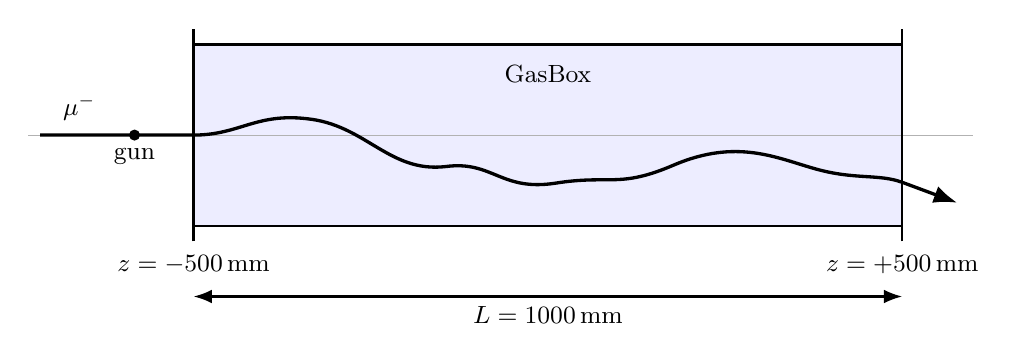
\begin{tikzpicture}[x=1cm,y=1cm,>=Latex,font=\small]
  \fill[blue!7] (2.3,-1.15) rectangle (11.3,1.15);
  \draw[thick] (2.3,-1.15) rectangle (11.3,1.15);
  \node at (6.8,0.78) {GasBox};

  \draw[gray!60] (0.2,0) -- (12.2,0);
  \draw[very thick,-{Latex[length=3mm]}] (0.35,0)
    -- (2.3,0) .. controls (2.9,0) and (3.1,0.30) .. (3.8,0.20) .. controls (4.5,0.10) and (4.8,-0.48) .. (5.5,-0.40) .. controls (6.1,-0.32) and (6.2,-0.72) .. (6.9,-0.61)
    .. controls (7.6,-0.50) and (7.7,-0.68) .. (8.4,-0.38) .. controls (9.2,-0.04) and (9.7,-0.29) .. (10.2,-0.43) .. controls (10.7,-0.57) and (11.0,-0.49) .. (11.3,-0.60) -- (12.0,-0.86);

  \node[above] at (0.85,0.06) {$\mu^-$};
  \node[below] at (1.55,-0.05) {gun};
  \fill (1.55,0) circle (2pt);

  \draw[thick] (2.3,-1.35) -- (2.3,1.35);
  \draw[thick] (11.3,-1.35) -- (11.3,1.35);
  \node[below] at (2.3,-1.40) {$z=-500\,\mathrm{mm}$};
  \node[below] at (11.3,-1.40) {$z=+500\,\mathrm{mm}$};

  \draw[<->,thick] (2.3,-2.05) -- (11.3,-2.05)
    node[midway,below] {$L=1000\,\mathrm{mm}$};
\end{tikzpicture}
\caption{Simulation geometry. The particle gun is located $10\,\mathrm{mm}$
upstream of the GasBox, and the beam travels in the $+z$ direction.}
\label{fig:geometry}
\end{figure}

\begin{figure}[H]
\centering
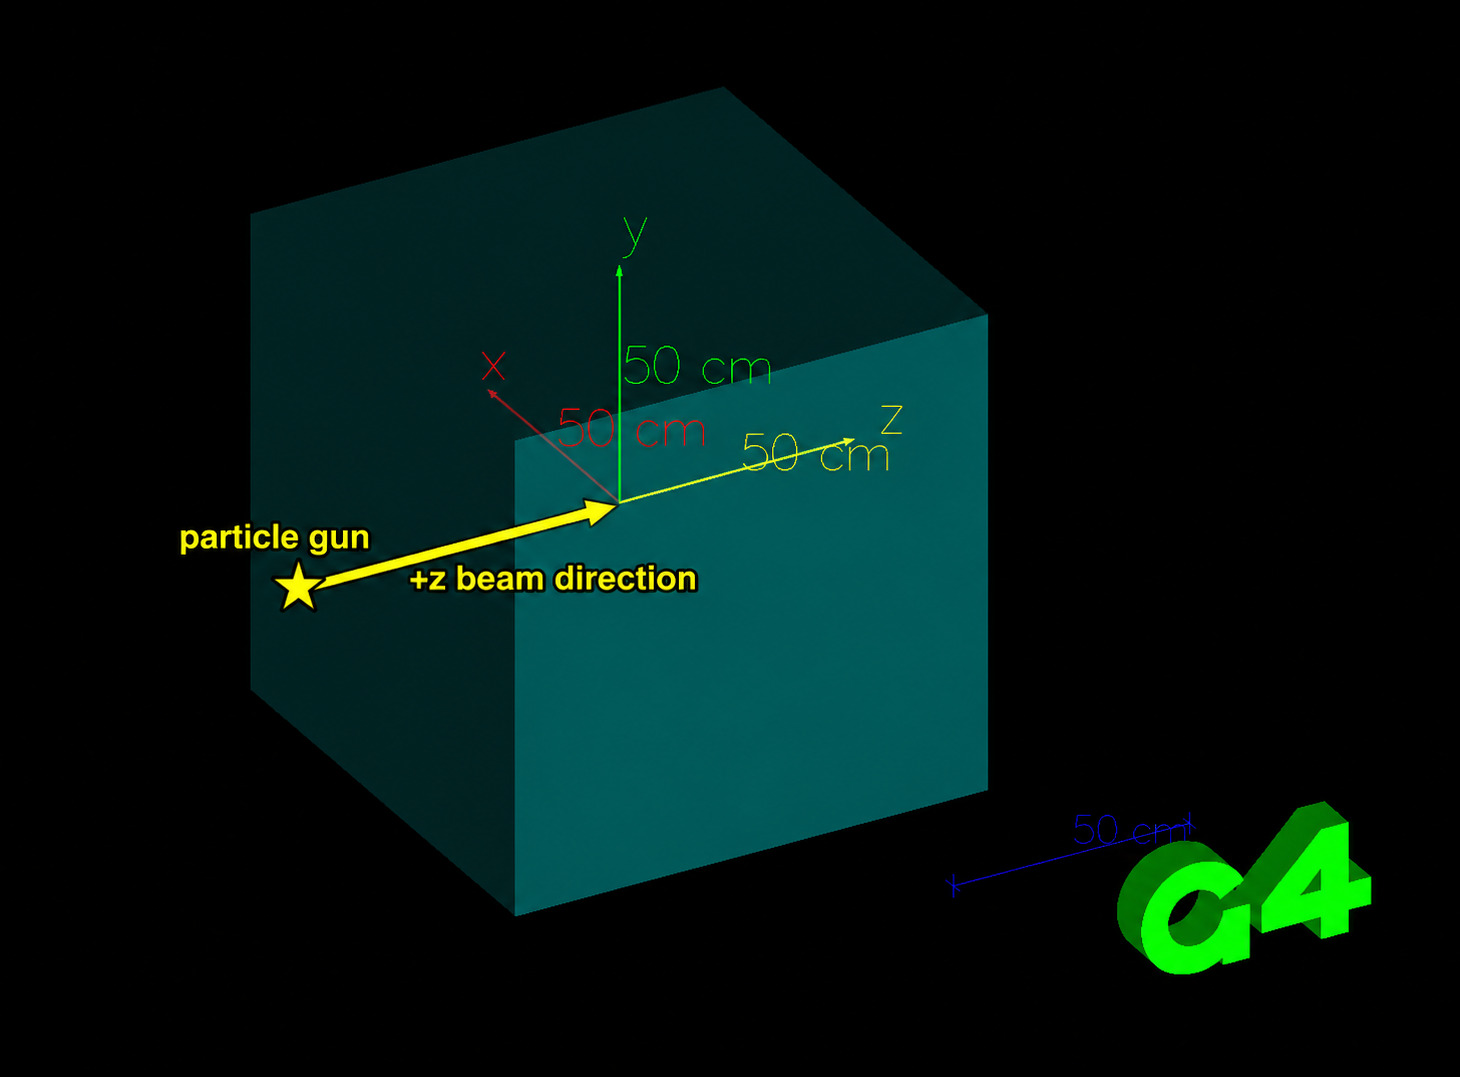
\includegraphics[width=0.61\textwidth]{geant4_geometry_annotated.png}
\caption{Geant4 visualization of the cubic GasBox. The yellow star marks the
particle-gun position, $10\,\mathrm{mm}$ upstream of the gas entrance, and the
yellow arrow shows the $+z$ beam direction into the gas. The coloured axes are
the Geant4 coordinate axes.}
\label{fig:geant4-geometry}
\end{figure}

Geant4 writes hit-level information and true boundary states to ROOT files. An
event is retained only when the primary particle is recorded at both the
upstream boundary and the downstream $z=+500\mm$ boundary. Side-exiting,
backscattered, and stopping tracks are excluded. A separate Python analysis
reads the ROOT trees, constructs event-level observables, and writes summary CSV
files used for the figures and tables.

\subsection{Signed projected observables}

For a nominal $+z$ beam, the projected changes in direction are
\begin{align}
\theta_x &= \operatorname{atan2}(p_{x,\mathrm{out}},p_{z,\mathrm{out}})
-\operatorname{atan2}(p_{x,\mathrm{in}},p_{z,\mathrm{in}}),\\
\theta_y &= \operatorname{atan2}(p_{y,\mathrm{out}},p_{z,\mathrm{out}})
-\operatorname{atan2}(p_{y,\mathrm{in}},p_{z,\mathrm{in}}),
\label{eq:theta}
\end{align}
and the entry-to-exit chord angles are
\begin{align}
\psi_x &= \operatorname{atan2}(x_{\mathrm{out}}-x_{\mathrm{in}},z_{\mathrm{out}}-z_{\mathrm{in}}),\\
\psi_y &= \operatorname{atan2}(y_{\mathrm{out}}-y_{\mathrm{in}},z_{\mathrm{out}}-z_{\mathrm{in}}).
\label{eq:psi}
\end{align}
All four variables are signed. In a symmetric geometry their means are
approximately zero, while their widths are positive. An unsigned
three-dimensional opening angle is non-negative and is not the variable
described by a zero-centred projected Gaussian.

\begin{figure}[H]
  \centering
  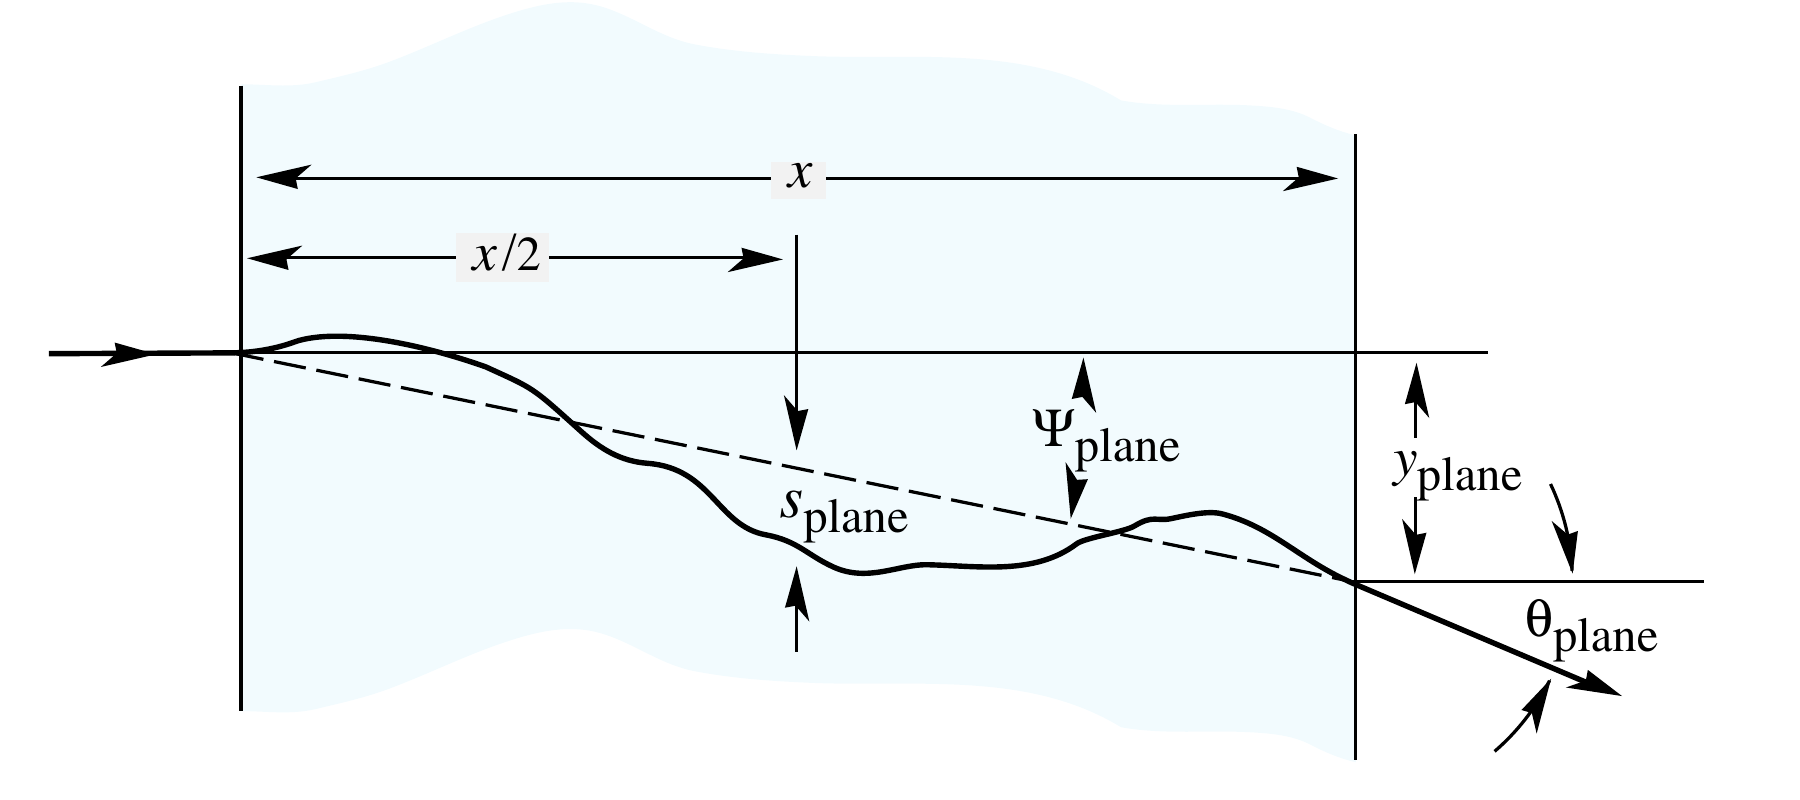
\includegraphics[width=0.93\textwidth]{pdg_multiple_scattering_geometry.png}
  \caption{PDG geometry for projected multiple scattering. The exit-direction
  angle is $\theta_{\mathrm{plane}}$, while $\psi_{\mathrm{plane}}$ is the
  angle of the chord joining the entrance and exit positions. Reproduced from
  Ref.~\cite{PDG2024}, Fig.~34.10.}
  \label{fig:pdg-geometry}
\end{figure}

\subsection{PDG width and width estimators}

For a particle with charge number $z$, momentum $p$, and speed $\beta c$
crossing a thickness $x$, the PDG gives the projected central width
\cite{PDG2024,LynchDahl1991}
\begin{equation}
\theta_0=\frac{13.6\MeV}{\beta pc}|z|\sqrt{\frac{x}{X_0}}
\left[1+0.038\ln\!\left(\frac{xz^2}{X_0\beta^2}\right)\right].
\label{eq:pdg}
\end{equation}
The quantity $\theta_0$ is a width of the approximately Gaussian central 98\%
of a signed one-plane distribution; it is not the angle of one particle.

For comparison with Eq.~\eqref{eq:pdg}, the analysis retains the central 98\%
and corrects the truncated RMS,
\begin{equation}
\sigma_{\mathrm{core}}=\frac{\operatorname{RMS}(\text{central 98\%})}{0.934553}.
\label{eq:core}
\end{equation}
For the Fermi--Eyges second-moment test, the full standard deviation is used,
\begin{equation}
\sigma_X=\sqrt{\frac{1}{N}\sum_{i=1}^{N}(X_i-\overline X)^2}.
\label{eq:rms}
\end{equation}
No Gaussian fit or tail truncation is applied in Eq.~\eqref{eq:rms}. The two
estimators answer different questions and are not interchanged.

\subsection{Motivation for the energy-loss study}

After correcting the angle and boundary definitions, the $50\MeVc$ muon
sample gave $\sigma_\theta/\sigma_\psi=2.0708\pm0.0023$, significantly above
the constant-scattering-power prediction $\sqrt{3}$. Checks of the event
statistics and physics list did not explain the difference, and both the muon
and proton control samples agreed with PDG at the few-percent level. However,
these muons lost 47.71\% of their mean kinetic
energy while crossing the gas. This large energy loss invalidates the
constant-scattering-power assumption and motivated the energy-dependent
Fermi--Eyges analysis below.

\subsection{Fermi--Eyges transport}

Let $s$ be the distance already travelled from the gas entrance and define the
projected scattering power $T(s)=d\langle\theta^2\rangle/ds$. Independent small
angular kicks give the Fermi--Eyges moments \cite{Eyges1948,Gottschalk2010}
\begin{align}
\operatorname{Var}(\theta)&=\int_0^L T(s)\,ds,\\
\operatorname{Var}(\psi)&=\frac{1}{L^2}\int_0^L(L-s)^2T(s)\,ds.
\label{eq:FE}
\end{align}
A kick at depth $s$ contributes fully to the exit direction but only acts over
the remaining lever arm $L-s$ when producing displacement. For constant
scattering power,
\begin{equation}
\operatorname{Var}(\theta)=T_0L,\quad
\operatorname{Var}(\psi)=\frac{T_0L}{3},\quad
\frac{\sigma_\theta}{\sigma_\psi}=\sqrt{3}.
\label{eq:sqrt3}
\end{equation}
This is a constant-scattering-power limit, not a universal value. To leading
order $T(s)\propto[\beta(s)p(s)]^{-2}$, so energy loss shifts scattering power
toward the exit. Late scattering changes $\theta$ strongly but has little lever
arm to change $\psi$, increasing the ratio above $\sqrt{3}$.

\section{Validation against PDG}

Before the final comparison, the gas composition, coordinate units, event
indexing, and true entry/exit boundaries were made consistent. These corrections
are included in all results below.

We used the Gaussian-equivalent width of the central 98\% of each signed
projected $\theta$ distribution, matching the PDG definition of $\theta_0$.
As a cross-check, we tested $200\MeVc$ muons and $1\GeVc$ protons. Different
momenta were chosen so that both samples could traverse the gas with limited
energy loss; this was therefore not a fixed-momentum comparison designed to
isolate particle type. The Geant4/PDG ratio ranged from 1.009 to 1.035 for
muons and from 1.036 to 1.064 for protons across four physics lists. Together,
these cross-checks showed only few-percent differences; neither control sample
showed a discrepancy large enough to explain the original result.
The later momentum and energy-loss study therefore used muons only. The full
comparison and angular distributions are available in Ref.~\cite{XuIndico}.

\section{Momentum dependence and energy loss}

The original $50\MeVc$ muon sample is not a constant-scattering-power test. Its
incident kinetic energy is $11.233\MeV$ and mean exit energy is $5.874\MeV$, a
loss of 47.71\%. Eleven momenta from $50\MeVc$ to $2\GeVc$ were therefore
simulated with one million generated muons at each point. Between 99.51\% and
99.99\% satisfied the downstream-boundary selection.

\begin{figure}[H]
\centering
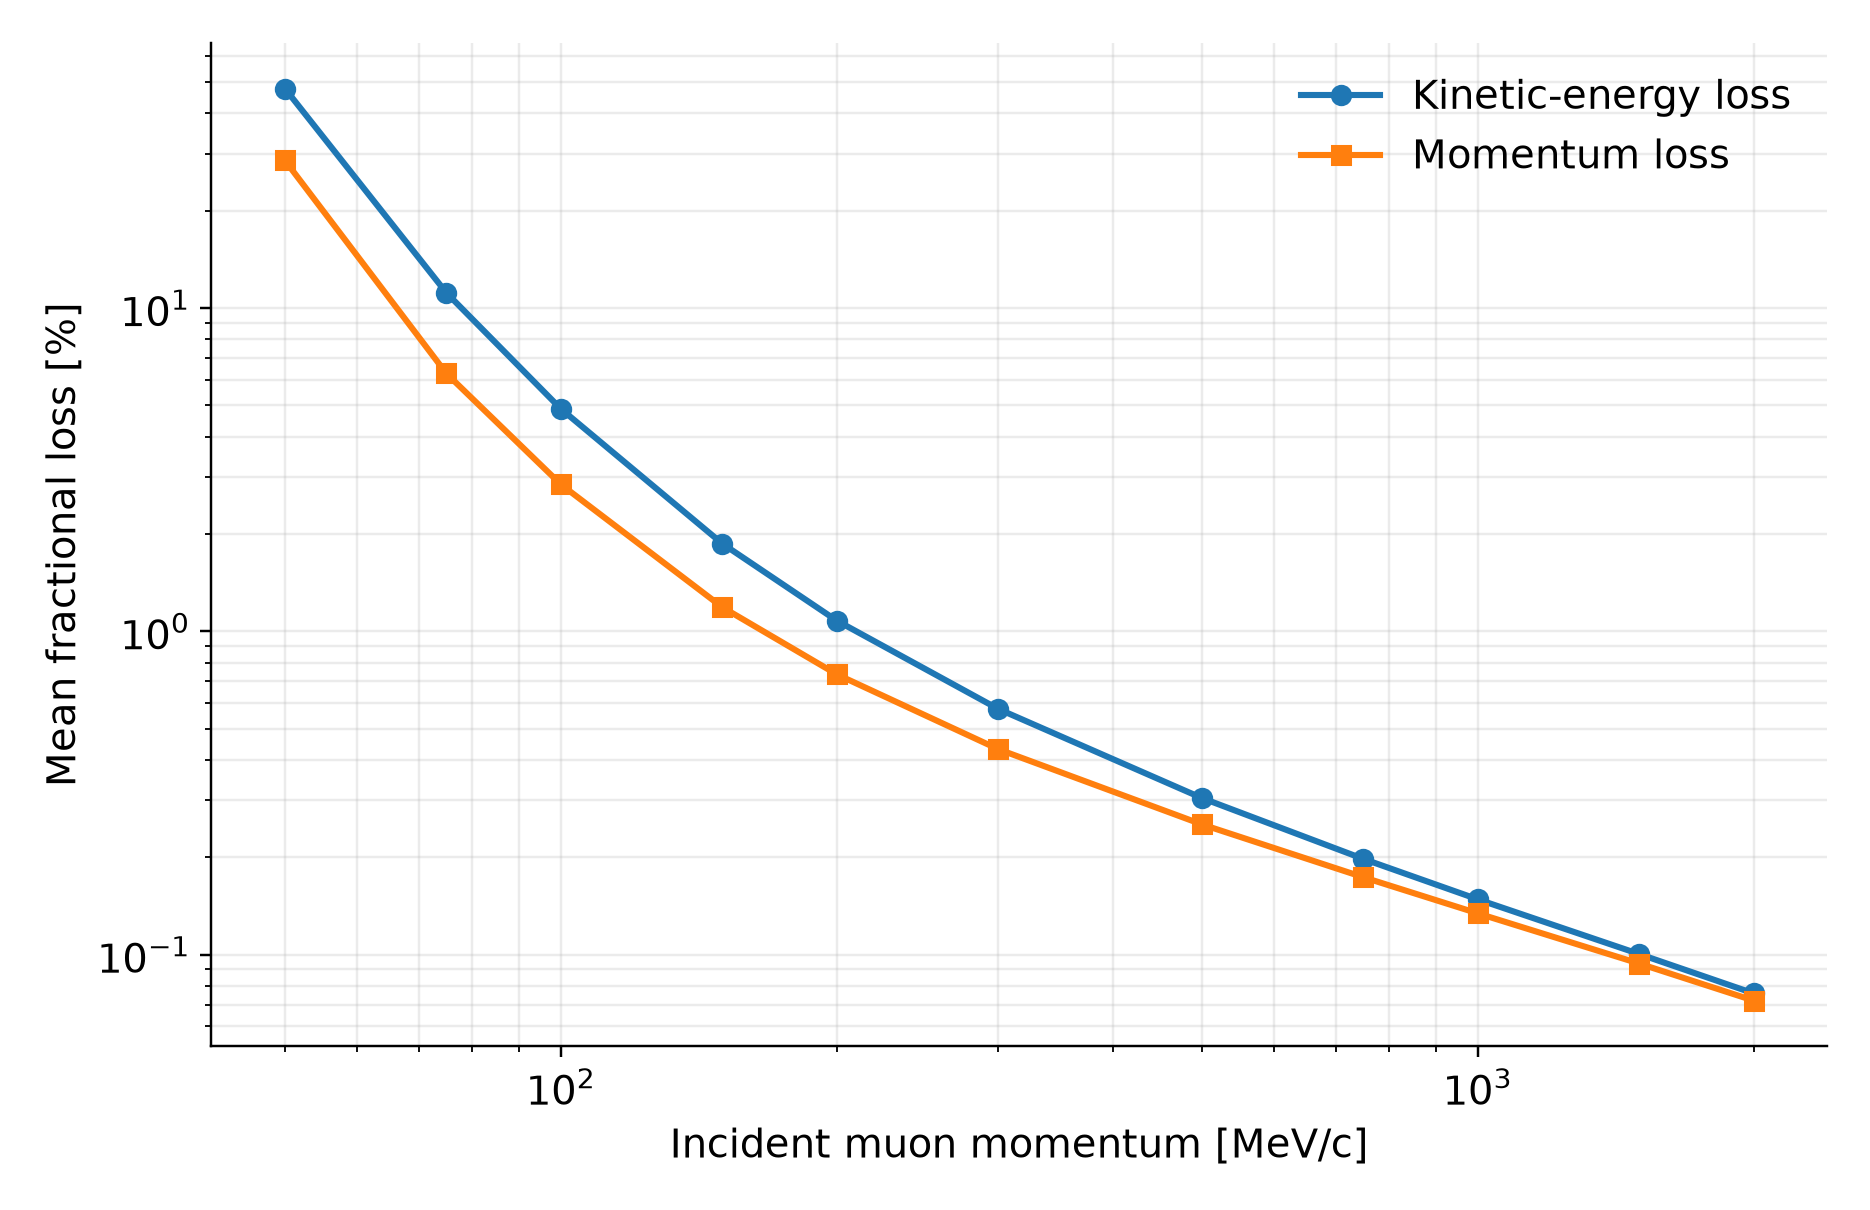
\includegraphics[width=0.86\textwidth]{energy_loss_vs_momentum.png}
\caption{Mean fractional kinetic-energy loss in the momentum scan.}
\label{fig:loss}
\end{figure}

\begin{figure}[H]
\centering
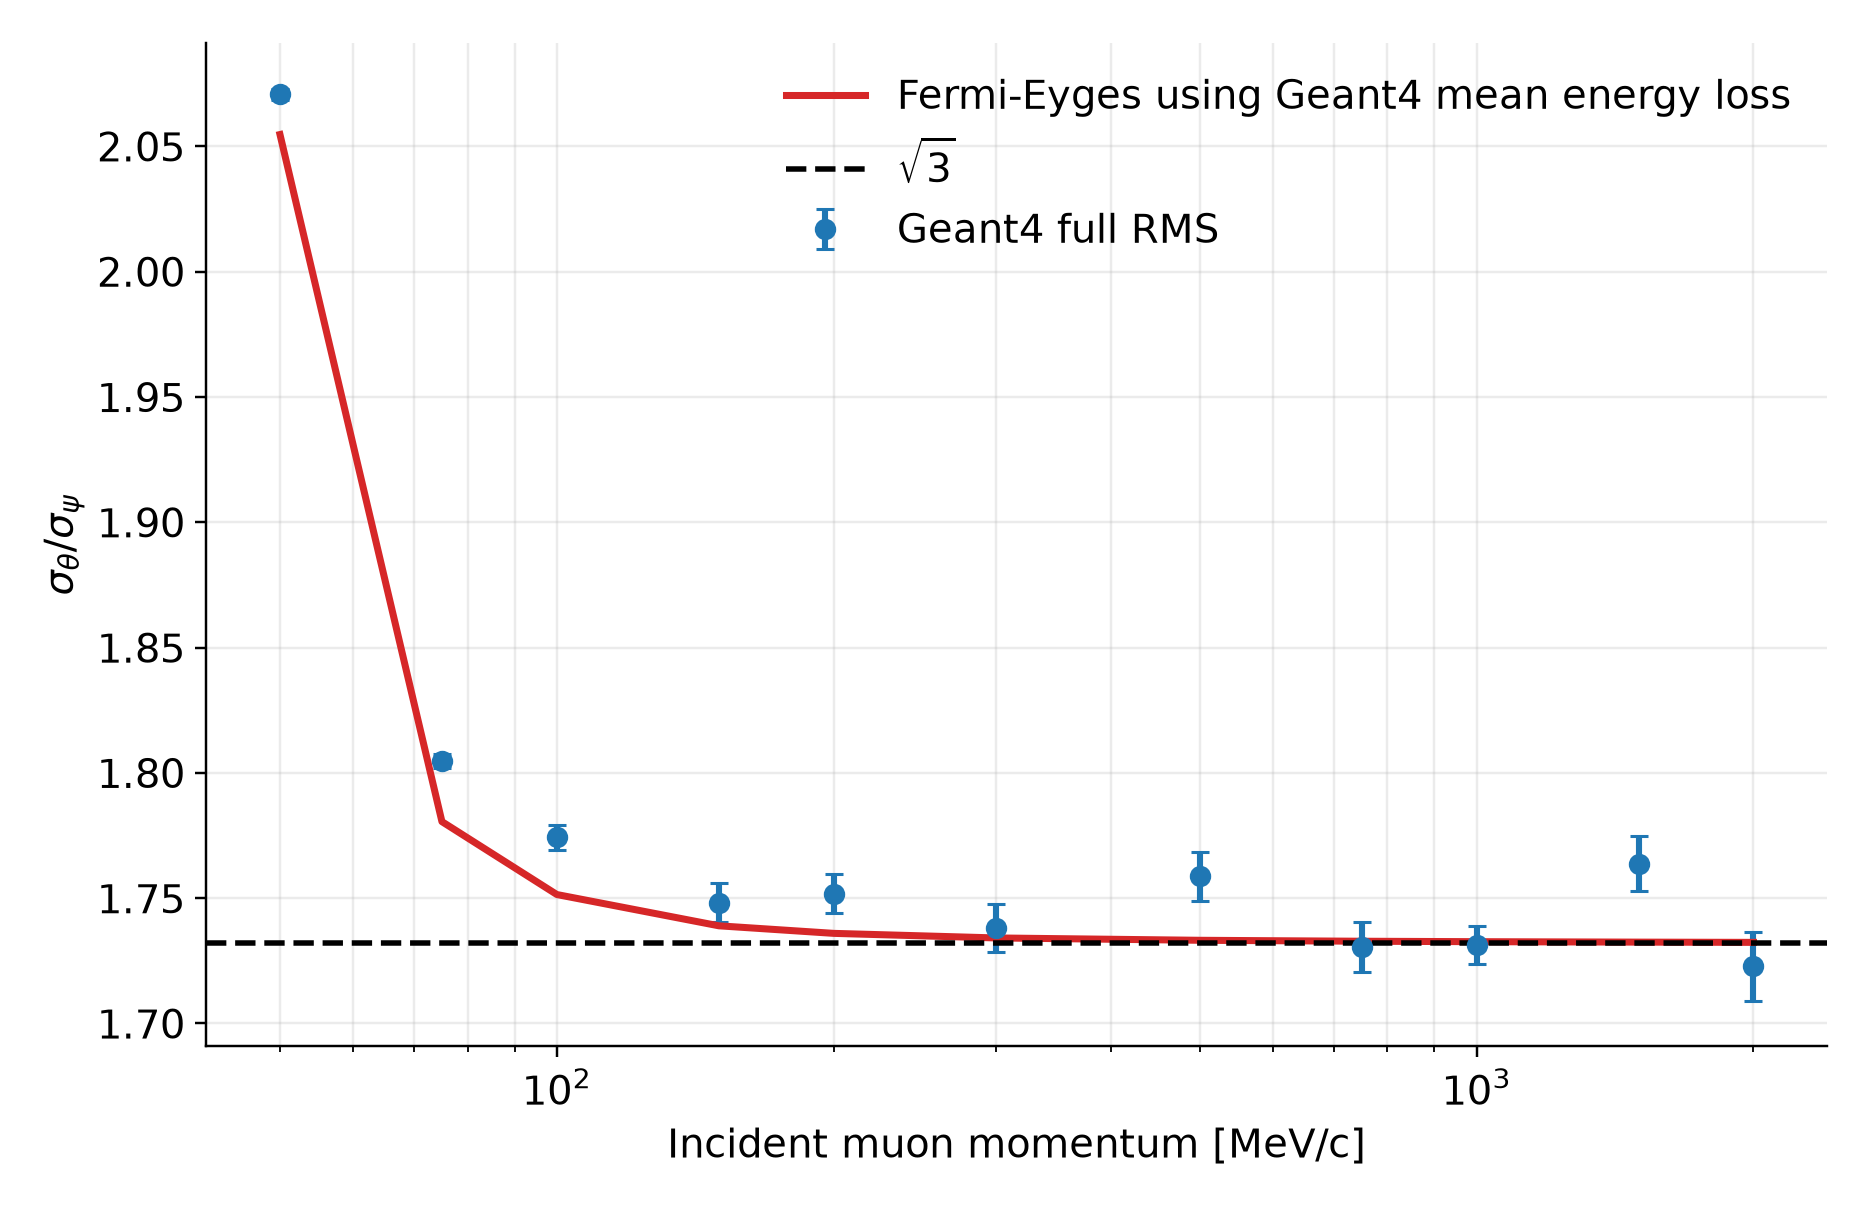
\includegraphics[width=0.92\textwidth]{ratio_vs_momentum.png}
\caption{Full-RMS ratio $\sigma_\theta/\sigma_\psi$ for $10^6$ generated
muons at each incident momentum. Blue points are Geant4 results with
block-resampling standard errors. The red curve is a Fermi--Eyges calculation
using the Geant4 mean entry and exit energies and is not a fit. The full RMS is
used here because the Fermi--Eyges relation is a relation between full second
moments; the central-98\% estimator is used separately for comparison with the
PDG core width $\theta_0$.}
\label{fig:ratio}
\end{figure}

For the red curve, the simulated endpoint energies define a linear mean profile,
\begin{equation}
K(u)=K_{\mathrm{in}}+(K_{\mathrm{out}}-K_{\mathrm{in}})u,\qquad u=s/L.
\end{equation}
Relativistic kinematics gives
\begin{equation}
p(u)=\sqrt{K(u)[K(u)+2m_\mu]},\qquad \beta(u)=\frac{p(u)}{K(u)+m_\mu}.
\end{equation}
The common material coefficient cancels in the ratio, so only
$T(u)\propto[\beta(u)p(u)]^{-2}$ is required:
\begin{equation}
R_{\mathrm{FE}}=\sqrt{\frac{\int_0^1T(u)\,du}{\int_0^1(1-u)^2T(u)\,du}}.
\label{eq:red}
\end{equation}
The integrals are evaluated numerically at each momentum; straight segments
only connect the independently calculated values.

\begin{table}[t]
\centering
\caption{Selected points from the one-million-event muon scan.}
\label{tab:scan}
\small
\begin{tabular}{rrrrr}
\toprule
$p_{\mathrm{in}}$ (MeV/$c$) & Accepted & KE loss & Geant4 ratio & $R_{\mathrm{FE}}$ \\
\midrule
50 & 995055 & 47.71\% & $2.0708\pm0.0023$ & 2.0547 \\
75 & 997544 & 11.14\% & $1.8046\pm0.0027$ & 1.7805 \\
100 & 998336 & 4.87\% & $1.7742\pm0.0049$ & 1.7515 \\
200 & 999201 & 1.08\% & $1.7518\pm0.0077$ & 1.7360 \\
1000 & 999852 & 0.148\% & $1.7315\pm0.0076$ & 1.7326 \\
2000 & 999927 & 0.0758\% & $1.7228\pm0.0137$ & 1.7324 \\
\bottomrule
\end{tabular}
\end{table}

The measured ratio decreases from $2.0708\pm0.0023$ at $50\MeVc$ to values
consistent with $\sqrt{3}$ at high momentum. The calculation reproduces the
scale and low-momentum trend. Residual differences may arise from energy-loss fluctuations,
non-Gaussian tails, finite-step transport, and event selection. High-momentum error bars remain
visible because a full RMS is tail-sensitive; more events reduce counting noise
but do not make the estimator tail-insensitive.

\section{Connection to the electron study}

This study does not test electrons directly. It provides a muon control sample
for checking the Geant4 code and the analysis method before a separate electron
study.

\section{Conclusions}

At high momentum, the simulated angular width agrees with the PDG prediction
at the few-percent level. The ratio $\sigma_\theta/\sigma_\psi$ approaches $\sqrt{3}$
when energy loss is small and increases at low momentum. The Fermi--Eyges
calculation shows that this increase is mainly caused by energy loss. Therefore,
the muon sample provides a useful control for the code and analysis method.

\section{Outlook}
The muon sample does not test the electron multiple-scattering model or
bremsstrahlung. A future electron study could compare simulations with and
without bremsstrahlung, using the same observables and width estimators as
the muon analysis. Grouping events by the kinetic-energy ratio
$K_{\rm out}/K_{\rm in}$ and comparing the full RMS with $\sigma_{\rm core}$
would help distinguish changes in the core from changes in the tails.
Muons and electrons could also be compared at similar $\beta p$, since
the PDG width scales approximately as $\theta_0 \propto 1/(\beta p)$
at fixed material thickness.

The Fermi--Eyges calculation still differs from Geant4 by about 0.02 in
$\sigma_\theta/\sigma_\psi$ at 75--200~MeV/$c$. We also evaluated the ratio
using recorded step-level energies and obtained nearly identical results,
so the linear energy approximation does not explain this difference.

\section*{Reproducibility and acknowledgements}

The Geant4 code and analysis files are stored in the UH Physics GitLab
\texttt{geant4-simulation} repository and are also available on GitHub
\cite{Repository}. The repositories contain the
\texttt{B1\_copy} application, build configuration, run macros, installation
instructions, and supporting project files needed to reproduce and extend the
simulation. The momentum-scan blue points come from event-level ROOT analysis;
the red values are computed by
\texttt{fermi\_eyges\_red\_line.py} from the same CSV endpoint-energy summary
and are not fitted.

The author thanks the members of the Vahsen research group for helpful discussions and a supportive research environment. 

\begin{thebibliography}{9}
\bibitem{PDG2024} D. E. Groom and S. R. Klein, ``Passage of Particles Through Matter,'' in S. Navas \emph{et al.} (Particle Data Group), \emph{Phys. Rev. D} \textbf{110}, 030001 (2024), Sec.~34.3. \href{https://doi.org/10.1103/PhysRevD.110.030001}{doi:10.1103/PhysRevD.110.030001}.
\bibitem{LynchDahl1991} G. R. Lynch and O. I. Dahl, ``Approximations to multiple Coulomb scattering,'' \emph{Nucl. Instrum. Methods Phys. Res. B} \textbf{58}, 6--10 (1991). \href{https://doi.org/10.1016/0168-583X(91)95671-Y}{doi:10.1016/0168-583X(91)95671-Y}.
\bibitem{Eyges1948} L. Eyges, ``Multiple Scattering with Energy Loss,'' \emph{Phys. Rev.} \textbf{74}, 1534--1535 (1948). \href{https://doi.org/10.1103/PhysRev.74.1534}{doi:10.1103/PhysRev.74.1534}.
\bibitem{Gottschalk2010} B. Gottschalk, ``On the scattering power of radiotherapy protons,'' \emph{Med. Phys.} \textbf{37}, 352--367 (2010). \href{https://doi.org/10.1118/1.3264177}{doi:10.1118/1.3264177}; \href{https://arxiv.org/abs/0908.1413}{arXiv:0908.1413}.
\bibitem{Geant4Toolkit} S. Agostinelli \emph{et al.}, ``Geant4---a simulation toolkit,'' \emph{Nucl. Instrum. Methods Phys. Res. A} \textbf{506}, 250--303 (2003). \href{https://doi.org/10.1016/S0168-9002(03)01368-8}{doi:10.1016/S0168-9002(03)01368-8}.
\bibitem{Geant4MSC} Geant4 Collaboration, ``Multiple Scattering,'' \emph{Physics Reference Manual}. \url{https://geant4.web.cern.ch/documentation/dev/prm_html/PhysicsReferenceManual/electromagnetic/elastic_scattering/msc.html}.
\bibitem{Repository} K. Xu, ``Geant4 Simulation,'' source code, build
instructions, and simulation macros. UH Physics GitLab:\newline
\url{https://uhhepvcs.phys.hawaii.edu/dcube/geant4-simulation}.\newline
GitHub:\newline
\url{https://github.com/Burning-Sunrise/geant4-simulation}.
\bibitem{Long2026} H. Long, ``Angular resolution update,'' TPC group meeting,
University of Hawai`i at M\=anoa, June 3, 2026. Internal presentation available
through the DCube Indico meeting record:
\url{https://indico.phys.hawaii.edu/event/2888/}.
\bibitem{XuIndico} K. Xu, ``Geant4 multiple-scattering updates,'' DCube group
meeting presentations, University of Hawai`i at M\=anoa. Presentation PDF and
supporting material:
\url{https://indico.phys.hawaii.edu/event/2965/}.
\end{thebibliography}
\end{document}
